\documentclass[12pt, oneside, openany]{article}
\usepackage[utf8]{inputenc}
\usepackage{polski}
\renewcommand*{\figurename}{Rys.}
\usepackage{graphicx}
\usepackage{float}
\usepackage{geometry}
\usepackage{subcaption}
\geometry{
	left=25mm,
	right=25mm,%
	bindingoffset=10mm, 
	top=25mm, 
	bottom=25mm}
\title{
	Eksploracyjna analiza danych \\
	Światowy program szczepień przeciwko COVID-19
}
\author{
	Marek Grudkowski 156587
	\\
	Kamil Kaczmarkiewicz 171701
}

\begin{document}

\maketitle

\section{Ogólny opis danych}

Zbiór danych dotyczy aktualnego postępu poszczególnych państw w szczepieniach przeciwko COVID-19. Zawiera on informacje pochodzące prawie ze wszystkich krajów na świecie podzielone na poszczególne dni. Program szczepień przeciwko COVID to w dobie pandemii niezwykle gorący temat. Naszym zdaniem warto się na nim skupić, gdyż może zawierać wiele ukrytych informacji, które mogą przydać się w walce z pandemią i przyspieszyć sam proces szczepień. 

\section{Cel eksploracji i kryteria sukcesu}

\newpage

\section{Charakterystyka zbioru danych}
Zbiór danych na stan dnia pisania tego sprawozdania zawiera ponad 13300 przykładów. Dane aktualizowane są zazwyczaj każdego dnia i pochodzą z wielu różnych źródeł. Zazwyczaj są nimi organy krajowe lub lokalne, czy międzynarodowe organizacje. Dla każdego przykładu podane jest źródło i jego adres internetowy, co daje możliwość weryfikacji w przypadku jakichkolwiek wątpliwości co do poprawności danych. Dane zapisane są w jednym pliku w formacie csv i podzielone są na następujące kolumny:
\begin{itemize}
\item \textbf{country} - kraj, dla którego podawane są informacje o szczepieniu, atrybut nominalny w postaci ciągu znaków
\item \textbf{iso\_code} - kod ISO dla danego kraju, atrybut nominalny w postaci ciągu znaków
\item \textbf{date} - data wprowadzenia danych, atrybut nominalny opisujący datę
\item \textbf{total\_vaccinations} - bezwzględna liczba wszystkich szczepień ochronnych w danym kraju, atrybut numeryczny (liczba naturalna)
\item \textbf{people\_vaccinated} - liczba osób która otrzymała szczepionkę (przy dwóch dawkach liczona jest $\times2$), atrybut numeryczny (liczba naturalna)
\item \textbf{people\_fully\_vaccinated} -  liczba osób, które otrzymały cały zestaw szczepień, atrybut numeryczny (liczba naturalna)
\item \textbf{daily\_vaccinations\_raw} - dla danej pozycji liczba szczepień dla tej daty/kraju, atrybut numeryczny (liczba naturalna)
\item \textbf{daily\_vaccinations} - dla danej pozycji liczba szczepień dla tej daty/kraju, atrybut numeryczny (liczba naturalna)
\item \textbf{total\_vaccinations\_per\_hundred} - stosunek liczby szczepień do całkowitej liczby ludności danego dnia w kraju, atrybut numeryczny wyrażany w procentach
\item \textbf{people\_vaccinated\_per\_hundred} - stosunek liczby osób zaszczepionych do całkowitej liczby ludności danego dnia w kraju, atrybut numeryczny wyrażany w procentach
\item \textbf{people\_fully\_vaccinated\_per\_hundred} - stosunek liczby osób uodpornionych do całkowitej liczby ludności danego dnia w kraju, atrybut numeryczny wyrażany w procentach
\item \textbf{daily\_vaccinations\_per\_million} - stosunek między liczbą szczepień a całkowitą liczbą ludności na bieżący dzień w kraju, dodania liczba rzeczywista
\item \textbf{vaccines} - rodzaje szczepionek wykorzystanych w danym kraju, atrybut nominalny, ciągi znaków rozdzielone ukośnikiem
\item \textbf{source\_name} - źródło informacji, atrybut nominalny, ciąg znaków
\item \textbf{source\_website} - strona internetowa źródła informacji, atrybut nominalny, ciąg znaków
\end{itemize}


\section{Wyniki eksploracyjnej analizy danych}



Podczas analizowania danych pierwszym etapem, było sprawdzenie w jakiej ilości występują wartości puste. Ku naszemu zaskoczeniu przykładów z takimi wartościami było naprawdę dużo. Wyniki tej operacji zliczającej takie przykłady poniżej 

\begin{table}[h]

\centering
\begin{tabular}{|l|c|}
\hline
\multicolumn{1}{|c|}{\textbf{Atrybut}} & \textbf{Brakujące wartości} \\ \hline
country                                & 0                           \\ \hline
iso\_code                              & 0                           \\ \hline
date                                   & 0                           \\ \hline
total vaccinations                     & 5390                        \\ \hline
people vaccinated                      & 6069                        \\ \hline
people fully vaccinated                & 8069                        \\ \hline
daily vaccinations raw                 & 6685                        \\ \hline
daily vaccinations                     & 226                         \\ \hline
total vaccinations per hundred         & 5390                        \\ \hline
people vaccinated per hundred          & 6069                        \\ \hline
people fully vaccinated per hundred    & 8069                        \\ \hline
daily vaccinations per million         & 226                         \\ \hline
vaccines                               & 0                           \\ \hline
source name                            & 0                           \\ \hline
source website                         & 0                           \\ \hline
\end{tabular}
\caption{Puste wartości w zbiorze danych}
\label{Tab:Tcr}
\end{table}


W tabeli można zauważyć, że liczba brakujących wartości dla atrybutów takich jak \textit{people\_fully\_vaccinated\_per\_hundred} są takie same jak dla \textit{people\_fully\_vaccinated}. Widać, że jest to para \textit{liczba bezwzględna - liczba względna}. Na 9 atrybutów, w których występują brakujące dane, 8 z nich tworzy właśnie takie pary. Bardzo możliwe, że te atrybuty mogą być od siebie liniowo zależne i są to po prostu przykłady opisujące momenty, kiedy program szczepień nie funkcjonował jeszcze w danym kraju. 
\\
\
\\
Cały zbiór przykładów jest podzielony na państwa, więc obliczenie korelacji między kolejnymi atrybutami dla wszystkich państw mogło by nie dać poprawnych wyników, gdyż dane z każdego kraju pochodzą z innego źródła. W celu uniknięcia tego błędu policzyliśmy współczynnik korelacji między poszczególnymi atrybutami dla każdego państwa osobno i z otrzymanych wartości sporządziliśmy histogram. Wyniki są zaprezentowane na wykresie poniżej. 
\\
\
\\
Widać więc, że wszystkie owe atrybuty są od siebie wręcz idealnie liniowo zależne, co potwierdza nasze przypuszczenia. Dzięki tej krótkiej analizie byliśmy w stanie podjąć decyzję o uzupełnieniu \textit{sparowanych} atrybutów zerami.



\begin{figure}
  \begin{subfigure}[t]{.45\textwidth}
    \centering
    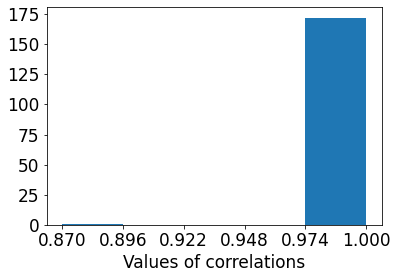
\includegraphics[width=\linewidth]{../img/null_column_diff1.png}
    \caption{Korelacja między dzienną liczbą wykonanych szczepień ogółem i na milion osób}
  \end{subfigure}
  \hfill
  \begin{subfigure}[t]{.45\textwidth}
    \centering
    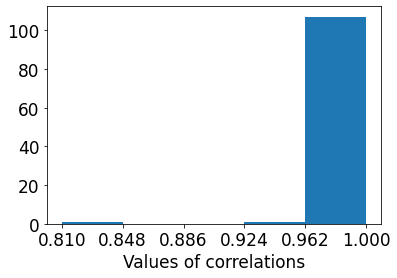
\includegraphics[width=\linewidth]{../img/null_column_diff2.png}
    \caption{Korelacja między liczbą ludzi w pełni zaszczepionymi ogółem i na 100 osób}
  \end{subfigure}

  \medskip

  \begin{subfigure}[t]{.45\textwidth}
    \centering
    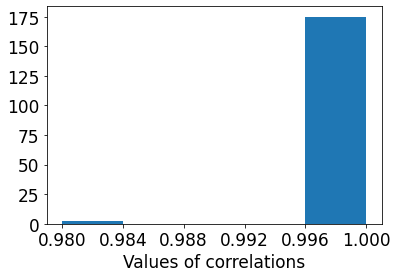
\includegraphics[width=\linewidth]{../img/null_column_diff3.png}
    \caption{Korelacja między liczbą ludzi którzy przyjęli choć jedną dawkę ogółem i na 100 osób}
  \end{subfigure}
  \hfill
  \begin{subfigure}[t]{.45\textwidth}
    \centering
    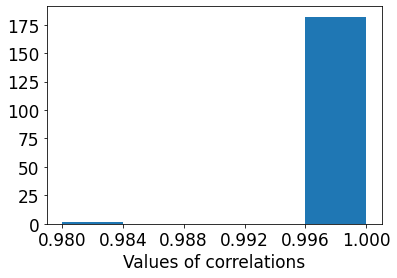
\includegraphics[width=\linewidth]{../img/null_column_diff4.png}
    \caption{Korelacja między liczbą wykonanych szczepień ogółem i na sto osób}
  \end{subfigure}
  \caption{Korelacje pomiędzy poszczególnym atrybutami zbioru}
\label{Rys:kor}
\end{figure}


Po wykonaniu tej operacji jedynym \textit{samotnym} atrybutem w jakim pozostały wartości \textit{null} jest \textit{daily\_vaccinations\_raw}. Jego nazwa wskazuje, że mógłby mieć powiązanie z atrybutem \textit{daily\_vaccinations}, ale żeby to stwierdzić, trzeba tak jak w poprzedniej sytuacji obliczyć korelację między tymi atrybutami. Rozkład wyznaczonych korelacji wśród państw ostatecznie odrzucił tą propozycję. Wynikowy histogram można zobaczyć na wykresie poniżej:


\begin{figure}[h]
\centering
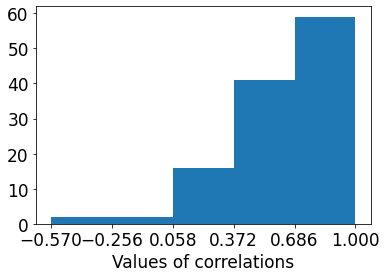
\includegraphics[scale=0.5]{../img/raw_corr.png} 
\label{Rys:kor}
\caption{Korelacja pomiędzy \textit{daily\_vaccinations\_raw} oraz \textit{daily\_vaccinations}}
\label{Rys:kor}
\end{figure}
\textbf{Co zostało do zrobienia:}
\begin{itemize}
\item opisać cele eksploracji i kryteria sukcesu
\item dodać heat map korelacji dla wszystkich państw
\item dodać heat map korelacji dla kilku przykładowych państw
\item opisać pochodzenie kolumny raw
\item dlaczego odrzucamy rozkład wartości bezwzględnych
\item wykresy pudełkowe dla wartości względnych
\item opisać wykresy pudełkowe (każdy osobno)
\item zaprezentować zmianę w czasie dla jednej kolumny
\item podsumowanie i wnioski
\end{itemize}




%Rozkłady wartości dla atrybutów 
%rozkłady wartości atrybutów, korelacje pomiędzy wartościami atrybutów
%wstępne ustalenia dotyczące zawartości zbioru 
%\section{Uwagi dotyczące jakości danych}
%dane brakujące, punkty oddalone, dane niespójne, dane niezrozumiałe,
%\section{Opis wyników eksploracji}
%w odniesieniu do celów eksploracji, czy dane są wystarczające, ewentualna rewizja celów

\end{document}
